\section{Dateien überschreiben}\abversion{2.9}
\label{sec:editor-allg-dateienueberschreiben}

Im Gegensatz zu vielen anderen (3D-)Anwendungen verwendet Loksim ein vollkommen offenes Dateiformat für sämtliche Addons. Zusätzlich sind Dateien nicht speziell an ein Package gebunden, sondern jedes einzelne Objekt, Textur, Führerstand, etc. kann im LoksimEdit geöffnet, betrachtet und sogar geändert werden.

Je nach \emph{Lizenz des Package} und der darin verwendeten Teile können Teile eines anderen Package auch - eventuell sogar in einer abgeänderten Form - in einem eigenen Package wiederverwendet werden. 

Bei einer Änderung einer fremden Datei ist jedoch \emph{immer eine Kopie anzulegen}, fremde Dateien dürfen \emph{niemals überschrieben} werden.

Lange Zeit wurde diese essentielle Übereinkunft technisch überhaupt nicht überprüft und nur eine sorgfältige Verwendung des LoksimEdit hat vor unabsichtlichem Überschreiben fremder Dateien geschützt. Mit Version 2.9 wurde hierfür zusätzlich eine technische Unterstützung eingführt, die das unabsichtliche Überschreiben fremder Dateien verhindern soll. Die Implementierung basiert dabei auf folgenden Grundsätzen:
\begin{itemize}
\item Jede Datei besitzt einen oder mehrere Autoren. Diese können im LoksimEdit über \emph{Datei - Eigenschaften} eingetragen werden. Mehrere Autoren können dabei mit einem \emph{;} (Strichpunkt) getrennt eingetragen werden. Es wird davon ausgegangen, dass nur eine Person welche als Dateiautor eingetragen ist, die Datei editieren sollte.
\item Im LoksimEdit ist der eigene Name (oder ein in der ''Loksim-Welt'' verwendetes Pseudonym) unter \emph{Datei - Editor Optionen - Sonstige - Standard Ersteller} eingetragen.
\item Wird eine Datei gespeichert ohne, dass ein Standard Ersteller in den Optionen eingetragen ist, wird eine Warnung angezeigt (\Fref{fig:editor-datei-ueberschreiben-empty})
\item Es wird eine Warnung angezeigt, falls versucht wird eine Datei ohne gesetztem Dateiautor zu speichern (\Fref{fig:editor-datei-ueberschreiben-empty})
\item Es wird gewarnt wenn versucht wird eine Datei zu speichern, bei welcher man nicht selbst als Dateiautor eingetragen ist (\Fref{fig:editor-datei-ueberschreiben-overwrite})
\item Falls beim Speichern einer Datei eine bestehende Datei überschrieben wird, wird überprüft ob bei der bestehenden Datei der Standard Ersteller als Dateiautor eingetragen ist. Ist er dies nicht, wird wiederum eine Warnung angezeigt (\Fref{fig:editor-datei-ueberschreiben-overwrite})
\end{itemize}

\begin{figure}
\centering
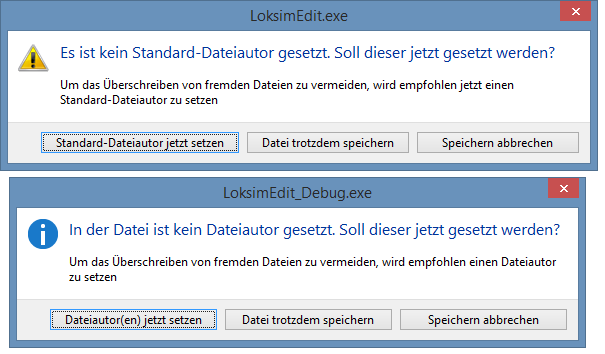
\includegraphics[width=1.0\textwidth]{editor/images/datei_ueberschreiben_empty.png}
\caption{Fehlermeldungen beim Speichern von Dateien ohne eingetragenem Standardersteller (oben) bzw. ohne eingetragenem Dateiautor (unten)}
\label{fig:editor-datei-ueberschreiben-empty}
\end{figure}

\begin{figure}
\centering
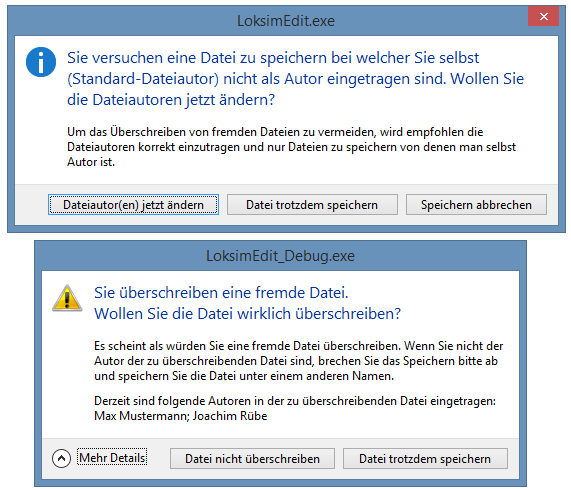
\includegraphics[width=1.0\textwidth]{editor/images/datei_ueberschreiben_overwrite.png}
\caption{Fehlermeldungen beim Speichern von Dateien bei denen man nicht selbst Dateiautor ist (oben) bzw. beim Überschreiben von fremden Dateien (unten)}
\label{fig:editor-datei-ueberschreiben-overwrite}
\end{figure}

Diese Lösung bietet keinen vollständigen Schutz vor dem Überschreiben fremder Dateien und schützt klarerweise überhaupt nicht vor dem Überschreiben von Dateien außerhalb des LoksimEdit. Ein vollständiger Schutz vor unbeabsichtigten Änderungen wäre wünschenswert, ist jedoch bei dem offenen Konzept von Loksim nicht einfach umzusetzen. Allerdings sollten die in Version 2.9 eingeführten Warnungen zumindest einen Teil der unabsichtlichen Änderungen verhindern.